\begin{problem}{Центральные  клетки}{стандартный ввод}{стандартный вывод}{1 секунда}{256 мегабайт}

Прямоугольник состоит из $N$x$M$ квадратных клеток. Назовём клетки на границе прямоугольника крайними. Расстоянием от какой-либо клетки до края назовём количеством перемещений, которое нужно сделать из данной клетки в соседнюю по стороне клетку, чтобы добраться от данной клетки до крайней клетки. Клетки с максимальным расстоянием до края, будем называть центральными. При это клетка может быть одновременно и крайней, и центральной.

На рисунке изображён прямоугольник для $N = 7$ и $M = 8$, в каждой клетке которого записано расстояние от этой клетки до края. У этого прямоугольника две центральных клетки.

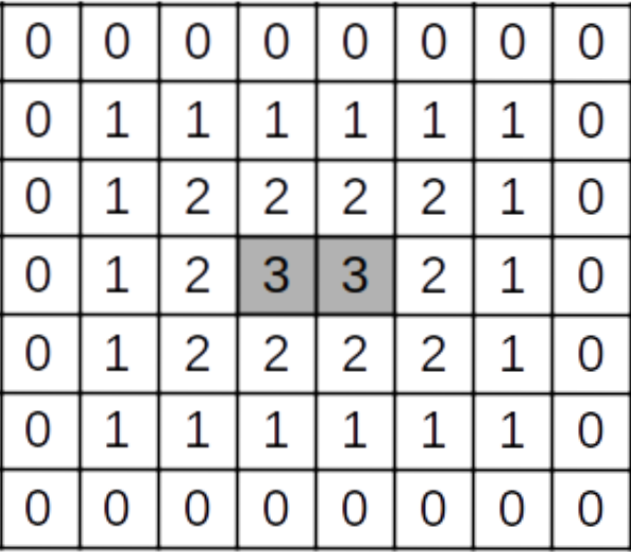
\includegraphics{IMG_0394.png}

По данным $N$ и $M$ определите количество центральных клеток в прямоугольнике.

\InputFile
Вводится два целых положительных числа записанных в разных строках, не превосходящих $10^9$ --- размеры прямоугольника.

\OutputFile
Вывести одно число --- количество центральных клеток в данном прямоугольнике.

\Example

\begin{example}
\exmpfile{example.01}{example.01.a}%
\end{example}

\end{problem}

